\section{Unifying Concurrency}\label{ha:UTCP}

\DRAFT{From TASE submission --- needs revising}

The Flexible and Strict PML semantics have in common that they
consider PML descriptions as denoting concurrent behaviour in the
presence of global shared state (resources).
They differ in the precise criterion used to determine when a particular task may actually run.
Our semantics is inspired closely by that of
UTPP \cite{DBLP:conf/icfem/WoodcockH02},
which translates a parallel program into an action system \cite{PODC::BackK1983},
whose semantics is given using UTP.
An action is viewed as a behaviour coupled with a guard that
establishes the conditions on observable state when that action may
begin to execute. An action system is a collection of such guarded actions,
that continually runs, with a non-deterministic choice being made whenever
multiple guards are enabled at the same time\cite{1976:book:dijkstra}.
In terms of UTP's lattice-theoretic approach,
the system is a distributed join (non-deterministic choice) of all its basic actions,
where a disabled (false) guard behaves the like the join unit value (top/miracle).
Or, in simpler predicate language, a disjunction of tasks as Designs,
with $\lnot ok$ as the unit.


Our semantics steps back a slight bit from the action-system formulation,
in that guards are de-emphasised, at least syntactically,
but we still have the distributed join, with disabled actions as unit.
We did this to reduce some of the mechanism associated with Designs,
so as to make the nature of the parallel semantics easier to see.
However, we expect our semantics can easily be ``poured'' back into a
full action system framework without any difficulty.

Our key motivation in stepping away from action systems,
and the UTPP formulation was to explore if we could eliminate one of the
sources of non-compositionality in that semantics,
namely that, while each basic statement had a starting label,
its semantics was defined in terms of that label,
and the labels of \emph{whatever statements came after it}.
We wanted to get better compositionality, so that the semantics of any construct was independent of its context,
and the semantics of any composite could be constructed from
the semantics of its components.
In the case of UTPP, it is not clear how much we have gained in terms
of calculational ease, but the UTP paradigm we have developed in order to
achieve this looks like it might be a framework for addressing a wider range of semantics where compositionality is difficult.



\subsection{UTCP Observables}

The key idea is that we use some observations to,
in effect, act as abstractions of the surrounding (local) context.
As actual context is built up by the use of language composites,
those observations are then instantiated in such a way
that either hides them as internal,
or lets them play an appropriate role at the higher level.

The theory we built uses predicate variables
to record observations of program behaviour
in two distinct ways:
\begin{enumerate}
  \item
    Making observations of dynamic state change,
    using un-decorated variables to record before-values,
    and dashed variables to denote the corresponding after-value,
    as is the norm in most UTP theories.
    We shall refer to these as \emph{dynamic observables}.
    In our theory we shall use $s$ to denote (shared) state
    and $ls$ to denote the current set of active labels.
    \begin{eqnarray*}
       s,s' &:& State
    \\ ls,ls' &:& \Set Label
    \end{eqnarray*}
  \item
    Some observations record context information that
    is propagated throughout a program.
    This information does not change during the lifetime of a program execution,
    and so only needs to be recorded using un-decorated variables.
    We shall call these \emph{static parameters}.
    In this theory we associate three static parameter with every construct: input and output labels ($in$,$out$)
    and a label generator ($g$).
    \begin{eqnarray*}
       in, out &:& Label
    \\ g &:& Gen
    \end{eqnarray*}
\end{enumerate}
The alphabet we use for a UTCP program ($P$, $Q$)  is
\begin{equation*}
  \alpha P = \setof{s,s',ls,ls',g,in,out}
\end{equation*}
However we will also talk about basic atomic actions ($A$,$B$)
that only affect the global state:
\begin{equation*}
  \alpha A = \setof{s,s'}
\end{equation*}

\subsection{Basic UTP Building Blocks}

The definition of the semantics of the UTCP language
constructs, and of $run$,
make use of the (almost) standard notions of skip,
sequential composition
and iteration in UTP.
The versions used here are slightly non-standard because we have
non-homogeneous relations,
where the static parameters have no dashed counterparts.
In essence we ignore the static parameters as far as flow-of-control is concerned:
\RLEQNSs{
   \Skip &\defs& s'=s \land ls'=ls
\\ P ; Q
   &\defs&
   \exists s_m,ls_m \bullet
\\ && \qquad P[s_m,ls_m/s',ls']
             \land
             Q[s_m,ls_m/s,ls]
\\ c * P &\defs& \mu L \bullet (P ; L) \cond c \Skip
\\ P \cond c Q &\defs& c \land P \lor \lnot c \land Q
}
Here, the definition of $\cond\_$ and $\_ * \_$ are entirely standard, of course.
We get the following very straightforward laws:
\RLEQNSs{
   \Skip;P  & = P = & P;\Skip
\\ s'=s ; A & = A = & A ; s'=s
\\ c * P    &   =   & (P ; c * P ) \cond c \Skip
}

\subsection{UTCP Semantics Overview}

We view the semantics of a concurrent program as being a collection
of all its atomic actions, each with an associated guard that enables
it, those guards being based on the presence or absence of labels
from the global label set ($ls$).
An enabled atomic action will run when its input label ($in$) is in $ls$,
at which point in time
it will make changes to the global shared variable state ($s$),
remove its $in$ label from $ls$,
and add its output label ($out$) to that set%
%(\figref{fig:atom-act:view})
.
A key point here to note is that every construct has both a input (start) label,
and a output (finish) label,
and its semantics is defined solely in terms of those.
The output label in particular,
belongs to the construct itself
and is not the label (or labels) of ``whatever comes after''.

%\begin{figure}[t!]
%  \centering
%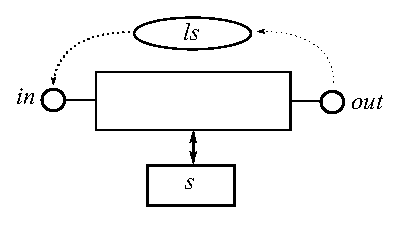
\includegraphics{images/atomic-action.eps}
%  \caption{Atomic Action view of the world}
%  \label{fig:atom-act:view}
%\end{figure}

\subsection{Atomic Action Semantics}

We use sets in two key ways:
checking for membership/subset inclusion;
and updating by simultaneously adding and removing elements:
%We use a shorthand (that views a set as its own collection
%of corresponding $n$-ary characteristic functions)
%as summarised in \figref{fig:short:membership}.
%The aim is to minimise displayed expression widths.
%\begin{figure}[t!]
%  \centering
%\begin{tabular}{|c|c|}
%\hline
%  Longhand & Shorthand
%\\\hline
%  $x \in S$ & $S(x)$
%\\\hline
%  $x \in \setof{y_1,\ldots,y_n} $ & $\setof{y_1,\ldots,y_n}(x)$
%\\\hline
%  $\setof{x_1,\ldots,x_n} \subseteq S$  & $S( x_1,\ldots,x_n)$
%\\\hline
%  $T \subseteq S$ & $S(T)$
%\\\hline
%  $\setof x$ &    $x$ (if context permits)
%\\\hline
%\end{tabular}
%  \caption{Set Membership Shorthands}
%  \label{fig:short:membership}
%\end{figure}
\RLEQNSs{
   A \ominus (B \rplby C) &\defs& (A \setminus B) \cup C
}
Let us consider an atomic state change operation,
viewed as a before-after relation on $State$:
\RLEQNSs{
   A(s,s') &:& State \rel State
}
We can lift this into an atomic concurrent action by adding in
the appropriate behaviour w.r.t to $in$, $out$, $ls$ and $ls'$:
\RLEQNSs{
    \A(A) &\defs& in \in ls \land A \land ls'=ls\ominus(\setof{in} \rplby\setof{out})
}
\noindent
To keep expression size manageable and clutter-free
we use a number of shorthands,
viz.,, $ls(in)$ for $ in \in ls$, $ls(a,b)$ for $\setof{a,b}\subseteq ls$,
$\ell$ for $\setof\ell$ (when it is clear a set is expected),
and $(a,b \rplby c,d)$ for ($\setof{a,b}\rplby \setof{c,d}$).
Given this shorthand we now write the atomic action semantics as:
\begin{equation*}
ls(in) \land A \land ls'=ls\ominus(in \rplby out)
\end{equation*}
A special case of this is the $Idle$ construct:
\RLEQNSs{
   Idle &\defs& \A(s'=s)
\\      &=& ls(in) \land s'=s \land ls'=ls\ominus(in \rplby out)
}
An atomic action has no need of the label generator $g$
so simply ignores it.
The situation with language composites is more complex, as we shall see.

\subsection{Composite Action Semantics}

For composite language constructs to work,
we require that the context of each component is somehow ``informed''
of how it is being situated.
We consider this the semantic responsibility of the composite itself,
and not something the components need to consider.

Let us consider sequential composition ($P \lseq Q$).
In effect, this operator has to glue its components
so that the $out$ label of the first corresponds to the $in$ label
of the second.
In effect it needs to generate a fresh label using $g$
and use this to replace the $out$ of $P$  and the $in$ of $Q$.
Then we need to split the generator in two and pass those bits
into $P$ and $Q$ for their own label generation needs.
The need for such generators arises because we can't use existential
quantification to hide a label,
because they need their presence in, or absence from, $ls$
to be globally visible.
We need these generators to have certain properties that ensure all
generated labels are unique,
and it is to this that we now turn.

\subsubsection{Label Generation}

We consider two operations that can be applied to a generator.
The first ($new$) returns a label, and a modified generator,
for further use.
The second ($split$) breaks a generator into two new generators
that will produce disjoint sets of labels.
To avoid long nested calls of $new$, $split$ and projections $\pi_1,\pi_2$,
we define the following terse label and generator expression syntax:
\RLEQNSs{
   g \in GVar && \text{Generator variables}
\\ G \in GExp &::=& g \mid G_{:} \mid G_1 \mid G_2
\\ L \in LExp &::=& \ell_G
}
Here $G_{:}$ denotes the generator left once $new$ has been run on $G$,
with $\ell_G$ denoting the label so generated.
Expressions $G_1$ and $G_2$ denote the two outcomes of applying $split$ to $G$.
We use $labs(G)$ to denote all the labels that $G$ can generate
and we require the following laws to hold:
\RLEQNSs{
   labs(G) &=& \setof{\ell_G} \cup labs(G_{:}) \cup labs(G_{1}) \cup labs(G_{2})
\\ \ell_G &\notin& labs(G_{:})
\\ \emptyset  &=& labs(G_{1}) \cap labs(G_{2})
}
The simplest model for a generator that satisfies the above constraints
is one that represents the label $\ell_G$ by the expression $G$ itself.
The reason for this shorthand is that without it we would have to write
something like the following
\begin{equation*}
\pi_1(new(\pi_2(new(\pi_2(split(\pi_2(new(\pi_1(split(g)))))))))).
\end{equation*}
instead of $\ell_{g1:2:}$.
%\begin{figure*}[t!]
%  \centering
%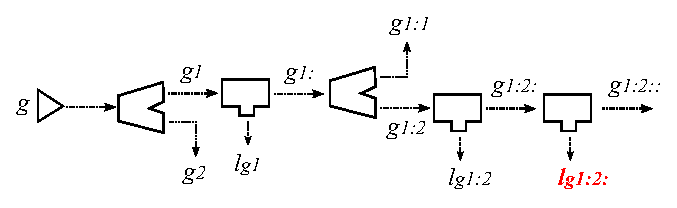
\includegraphics{images/label-gen-example.eps}
%  \caption{Label generation example: $\ell_{g1:2:}$}
%  \label{fig:label-gen-xampl}
%\end{figure*}
%(See \figref{fig:par-prog:view})

%\begin{figure}[t!]
%  \centering
%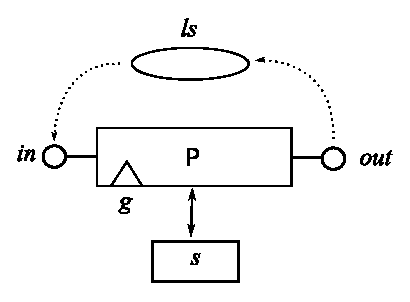
\includegraphics{images/parallel-program.eps}
%  \caption{Concurrent Program view of the world}
%  \label{fig:par-prog:view}
%\end{figure}


\subsubsection{Sequential Composition}





For sequential composition ($P \lseq Q$) we use the generator $g$
first to create the label ($\ell_g$) that connects $out$ of $P$ to $in$ of $Q$,
and then we split the leftover generator ($\g{:}$)
and give one ($\g{:1}$) to $P$, and the other ($\g{:2}$) to $Q$%
%(\figref{fig:seq-actual:view})
.
We simply use substitution to replace the static parameters
of both $P$ and $Q$ by the appropriate generator and label expressions.
\RLEQNSs{
    P \lseq Q &\defs& P[\g{:1},\ell_g/g,out] \lor Q[\g{:2},\ell_g/g,in]
}
We group the appropriately transformed components
using disjunction, as per the UTPP and action systems approach.
%\begin{figure*}[t!]
%  \centering
%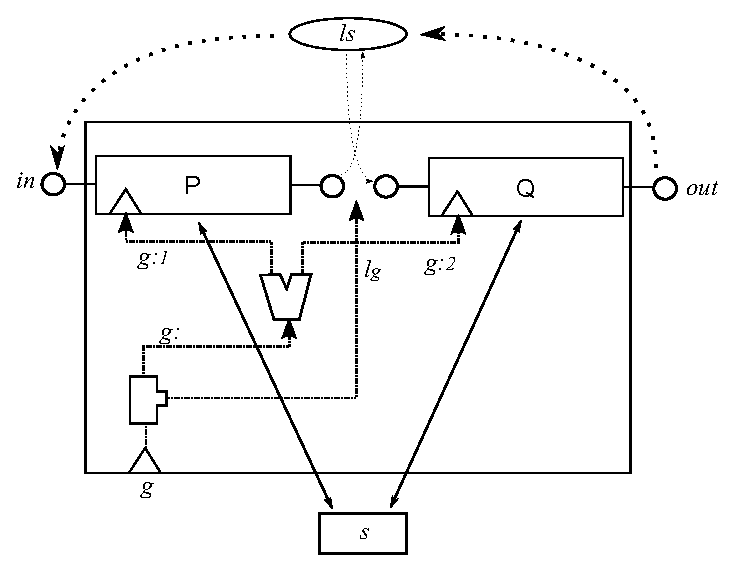
\includegraphics{images/seq-comp-actual.eps}
%  \caption{Sequential Composition actual construction}
%  \label{fig:seq-actual:view}
%\end{figure*}


\subsubsection{Parallel Composition}



Initially, parallel composition appears easy:
simply split the generator and pass to each part,
but leave $in$ and $out$ alone:
\[
  P[\g1/g] \lor Q[\g2/g]
\]
However this does not work---consider if $P$ is atomic and runs first:
the $in$ is removed from, and $out$ added to $ls$, effectively disabling $Q$.
Instead we need to seperate out the $in$ and $out$ labels of $P$ and $Q$,
and introduce two new atomic ``actions'': one to split $in$  into two new
start labels; and another to merge finish labels into $out$.
These split and merge actions do not alter state $s$.
We need to split the generator ($\g1,\g2$)
and generate two labels
(start: $\ell_{g1},\ell_{g2}$,
 finish: $\ell_{g1:},\ell_{g2:}$)
from each before passing them ($\g{1::},\g{2::}$) into $P$ and $Q$.
\RLEQNSs{
   Split(\ell_a,\ell_b)
   &\defs&
         ls(in)
   \land s'=s
   \land ls'=ls\ominus(in \rplby \ell_a,\ell_b)
\\ Merge(\ell_a,\ell_b)
   &\defs&
         ls(\ell_{g1:},\ell_{g2:})
   \land s'=s
\\ && {} \land ls'=ls\ominus(\ell_a,\ell_b \rplby out)
}
So, the parallel composition is a disjunction between
$Split(\ell_{g1},\ell_{g2})$,
the two components with appropriate re-labelling,
and $Merge(\ell_{g1:},\ell_{g2:})$%
%(\figref{fig:par-actual:view})
.
%\begin{figure}[t!]
%  \centering
%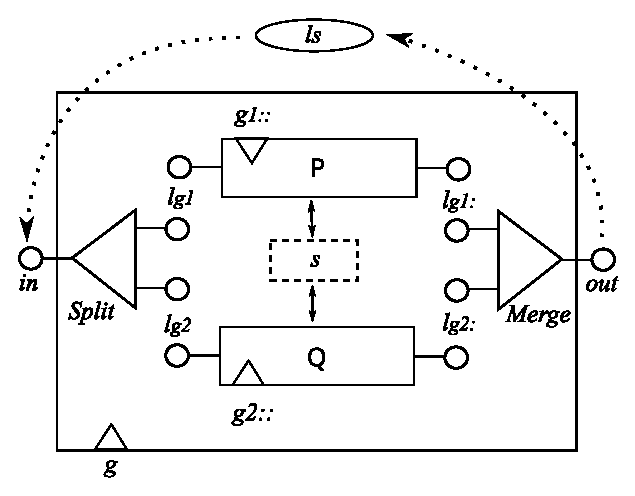
\includegraphics[scale=0.8]{images/par-comp-actual.eps}
%  \caption{
%     Parallel Composition actual construction (omitting generators).
%     The $s$ box is dashed to emphasise its global nature,
%     \emph{i.e.}, that it lies outside/under the program box
%  }
%  \label{fig:par-actual:view}
%\end{figure}
\RLEQNSs{
    P \parallel Q
    &\defs&
    ~~~~ Split(\ell_{g1},\ell_{g2})
\\&& {} \lor P[\g{1::},\ell_{g1},\ell_{g1:}/g,in,out]
\\&& {} \lor Q[\g{2::},\ell_{g2},\ell_{g2:}/g,in,out]
\\&& {} \lor Merge(\ell_{g1:},\ell_{g2:})
}

\subsubsection{Conditionals}

For the conditional, as only one arm will run, we can share $out$,
but we need a split on $in$ that uses the condition $c$.
\RLEQNSs{
   Cond(\ell_a,c,\ell_b)
   &\defs&
         ls(in)
   \land s'=s
\\ && {} \land ls'=ls\ominus(in \rplby \ell_a \cond c \ell_b)
}
So we split the generator ($\g1,\g2$) and produce one start label from each
($\ell_{g1},\ell_{g2}$), and then pass the two remaining generators
($\g{1:},\g{2:}$)
into $P$ and $Q$ as appropriate.
We then have a conditional-split ``action'' that
converts $in$ into $\ell_{g1}$ or $\ell_{g2}$ as determined by the condition%
%(\figref{fig:cond-actual:view})
.
%\begin{figure}[t!]
%  \centering
%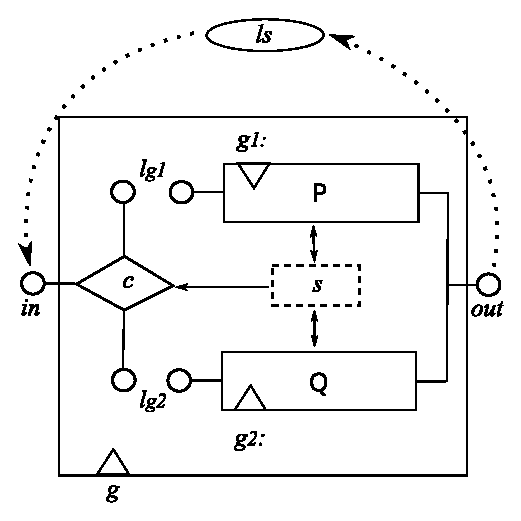
\includegraphics[scale=0.8]{images/conditional-actual.eps}
%  \caption{Conditional actual construction (omitting generators)}
%  \label{fig:cond-actual:view}
%\end{figure}
\RLEQNSs{
    P \lcond c Q
    &\defs& Cond(\ell_{g_1},c,\ell_{g2})
\\&& {} \lor P[\g{1:},\ell_{g1}/g,in] \lor Q[\g{2:},\ell_{g2}/g,in]
}

\subsubsection{Iteration}


Iteration is quite straightforward,
as we view it as a conditional loop unrolling%
%(\figref{fig:iter-actual:view})
.
We generate a label ($\ell_g$) for the entry-point to $P$,
pass the remaining generator ($\g:$) into $P$
and identify $P$'s exit with the loop entry.
%\begin{figure}[t!]
%  \centering
%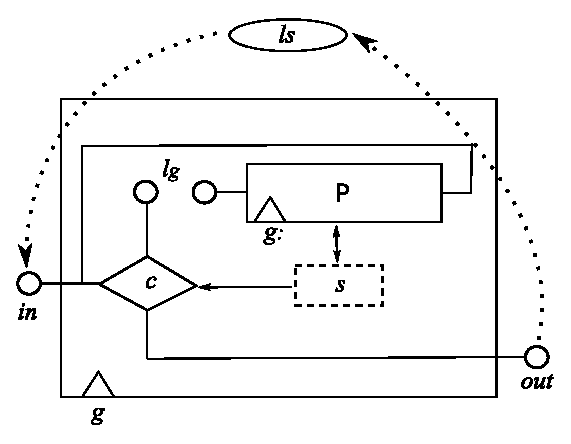
\includegraphics[scale=0.8]{images/iteration-actual.eps}
%  \caption{Iteration actual construction (omitting generators)}
%  \label{fig:iter-actual:view}
%\end{figure}
\RLEQNSs{
   c \wdo P
   &\defs&
    ls(in) \land s'=s \land ls'=ls\ominus(in \rplby \ell_{g} \cond c out)
\\&& {} \lor P[\g{:},\ell_{g},in/g,in,out]
}

\subsection{Running a concurrent program}

So far the semantics we have written simply views a concurrent program
as a big disjunction of atomic actions that use labels in a particular way.
This is a very static view of the program meaning.
To get a dynamic semantics we need to embed the above static
view, with appropriate initialisation,
into a loop that repeatedly runs the static disjunction
until a suitable (label-based) termination condition is reached.
We shall denote by $run(P)$ the result of adding dynamism
to a static view $P$ in this way.
We produce $run(P)$ by using the generator $g$
to create two labels $\ell_g$ and $\ell_{g:}$,
and then pass the remaining generator $\g{::}$
into the (static) program body $P$.
We use $\ell_g$ to replace $in$,
and $\ell_{g:}$ to replace $out$ in $P$.
We put this into a loop which keeps running so long as $\ell_{g:}$
is not in $ls$.
\RLEQNSs{
   run(P)
   &\defs&
   (\lnot ls(\ell_{g:}) * P[\g{::},\ell_{g},\ell_{g:}/g,in,out])[\ell_g/ls]
}
At the very top level, we initialise $ls$ to be $\setof{\ell_g}$.
Note that we cannot push this into the substitutions on $P$,
otherwise all that happens is that the first enabled action keeps running.

Space precludes us here from showing detailed calculations,
but we have obtained the following results which have
contributed to the validation of this semantics.
Here the lefthand side shows $P$, while the righthand side
shows a calculation of the expansion $run(P)$
\RLEQNSs{
   Idle
   &\stackrel{run}{\rightarrow}&
   s'=s \land ls'=\ell_{g:}
\\ \A(A)
   &\stackrel{run}{\rightarrow}&
   A \land ls'\stackrel{run}{\rightarrow}\ell_{g:}
\\ \A(A) \lseq \A(B)
   &\stackrel{run}{\rightarrow}&
    ( A \seq B ) \land ls'\stackrel{run}{\rightarrow}\ell_{g:}
\\ \A(A) \parallel \A(B)
   &\stackrel{run}{\rightarrow}&
    (( A \seq B ) \lor ( B \seq A))\land ls'\stackrel{run}{\rightarrow}\ell_{g:}
\\ \A(A) \lcond c \A(B)
   &\stackrel{run}{\rightarrow}&
    ((c \land A ) \lor ( \lnot c \land B ))\land ls'\stackrel{run}{\rightarrow}\ell_{g:}
}
Note that in each case we get a final result in terms of the
atomic action on $s$ only,
plus an assertion that we have terminated.
For iteration we show a partial calculation
of $run(c \wdo \A(B))$ with result:
\RLEQNSs{
 && \lnot c \land s'\stackrel{run}{\rightarrow}s             \land ls'\stackrel{run}{\rightarrow}\ell_{g:}
\\ &\lor&       c \land B \land \lnot c' \land ls'\stackrel{run}{\rightarrow}\ell_{g:}
\\ &\lor& (~c \land B \land c' \land ls'\stackrel{run}{\rightarrow}\ell_{g::}
\\ && \quad{};{} \A(B)[\g{:::},\ell_{g::},\ell_g,\ell_{g::}/g,in,out,ps]
\\ && \quad{};{} \lnot ls(\ell_{g:}) *
\\ && \qquad (c \wdo \A(B))
\\ && [\g{:::},\ell_{g::},\ell_g,\ell_{g::}/g,in,out,ps]
}
Here we see the result
of performing zero or one iteration, which also mentions only state,
plus a third case that captures the second and subsequent iterations.
In particular there is no mention in the final result of $in$ or $out$.

The semantics of $run(c \wdo \A(A))$ we expect to have a terminating part
and a non-terminating part:
\RLEQNSs{
 && (\bigvee_{i \in \Nat} A^i ) \land \lnot c \land ls'=\setof{\ell_{g:}}
       \lor A^\omega \land c \land \ell_{g:} \notin ls'
\\ \WHERE & & A^0 = s'=s
\\        & & A^{n+1} = A ; A^n
\\        & & A^\omega = \mbox{infinite sequence of $A$s}
}
From the above we can see that a possible interpretation of our semantics as a
Design is
\RLEQNSs{
   ok &\defs&  \ell_g \in ls
\\ ok' &\defs&  \ell_{g:} \in ls'
}

\subsection{Healthiness Conditions}

Our semantics has been designed
to ensure that,
for any program $P$ with alphabet $s,s',ls,ls',in,out,g$,
during any program run,
the following four predicates
are mutually exclusive, and exhaustive:
\RLEQNS{
   (\setof{in,out}\cup lab(g)) \cap ls &=& \emptyset
                                    \label{eqn:asleep}
\\ in &\in& ls                      \label{eqn:just-started}
\\ lab(g) \cap ls &\neq& \emptyset  \label{eqn:running}
\\ out &\in& ls                     \label{eqn:just-stopped}
}
This observations comprise a key healthiness condition
that ensures that all  components get executed
in a coherent manner, moving from a ``sleeping state'' (\ref{eqn:asleep}),
to being just started (\ref{eqn:just-started}),
running (\ref{eqn:running}),
just finished (\ref{eqn:just-stopped}),
and then possibly back to being asleep.
We can accordingly define some program status predicates as follows:
\RLEQNSs{
   started(P)
   &\defs&
   in \in ls
\\ running(P)
   &\defs&
   \setof{in,out} \cap ls = \emptyset
   \land
   \exists \ell \in ls \bullet \ell \in labs(g)
\\ stopped(P) &\defs& out \in ls
}
Note that $running(\A(A))$ is always false,
as an atomic action effectively occurs instantly.
